% !TeX root = ../thesis.tex
%\begin{appendices}
  % !TeX root = ../../thesis.tex
\section{Results of running deviceQuery}\label{app:deviceQuery}
\RecustomVerbatimCommand{\VerbatimInput}{VerbatimInput}%
{fontsize=\footnotesize,
 %
 frame=lines,  % top and bottom rule only
 framesep=2em, % separation between frame and text
 commandchars=\|\(\), % escape character and argument delimiters for
                      % commands within the verbatim
 commentchar=*        % comment character
}
\VerbatimInput{sections/appendix/deviceQuery.txt}
  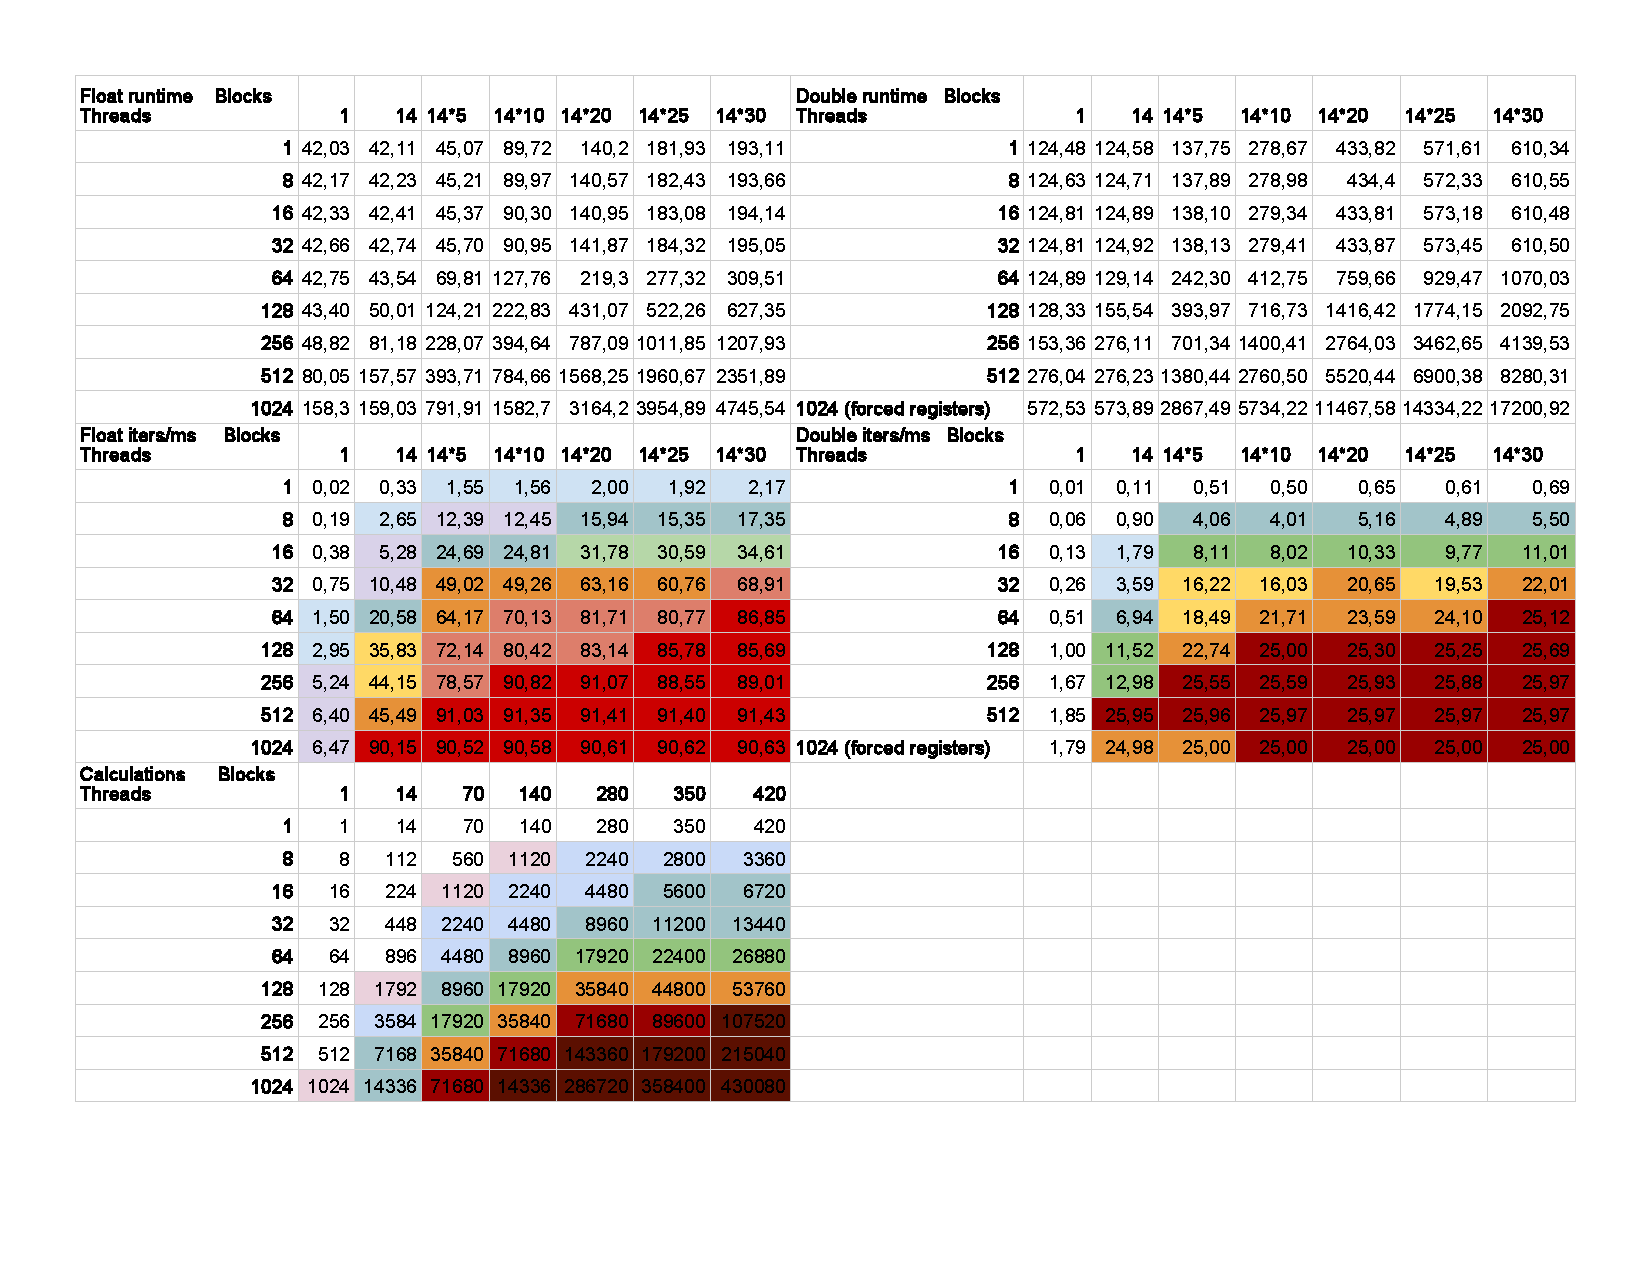
\includepdf[pages=1,angle=90,pagecommand={\section{CUDA C Performance Test}\label{app:cuda_runtimes}}, frame,scale=0.65]{sections/appendix/cuda_runtimes.pdf}
  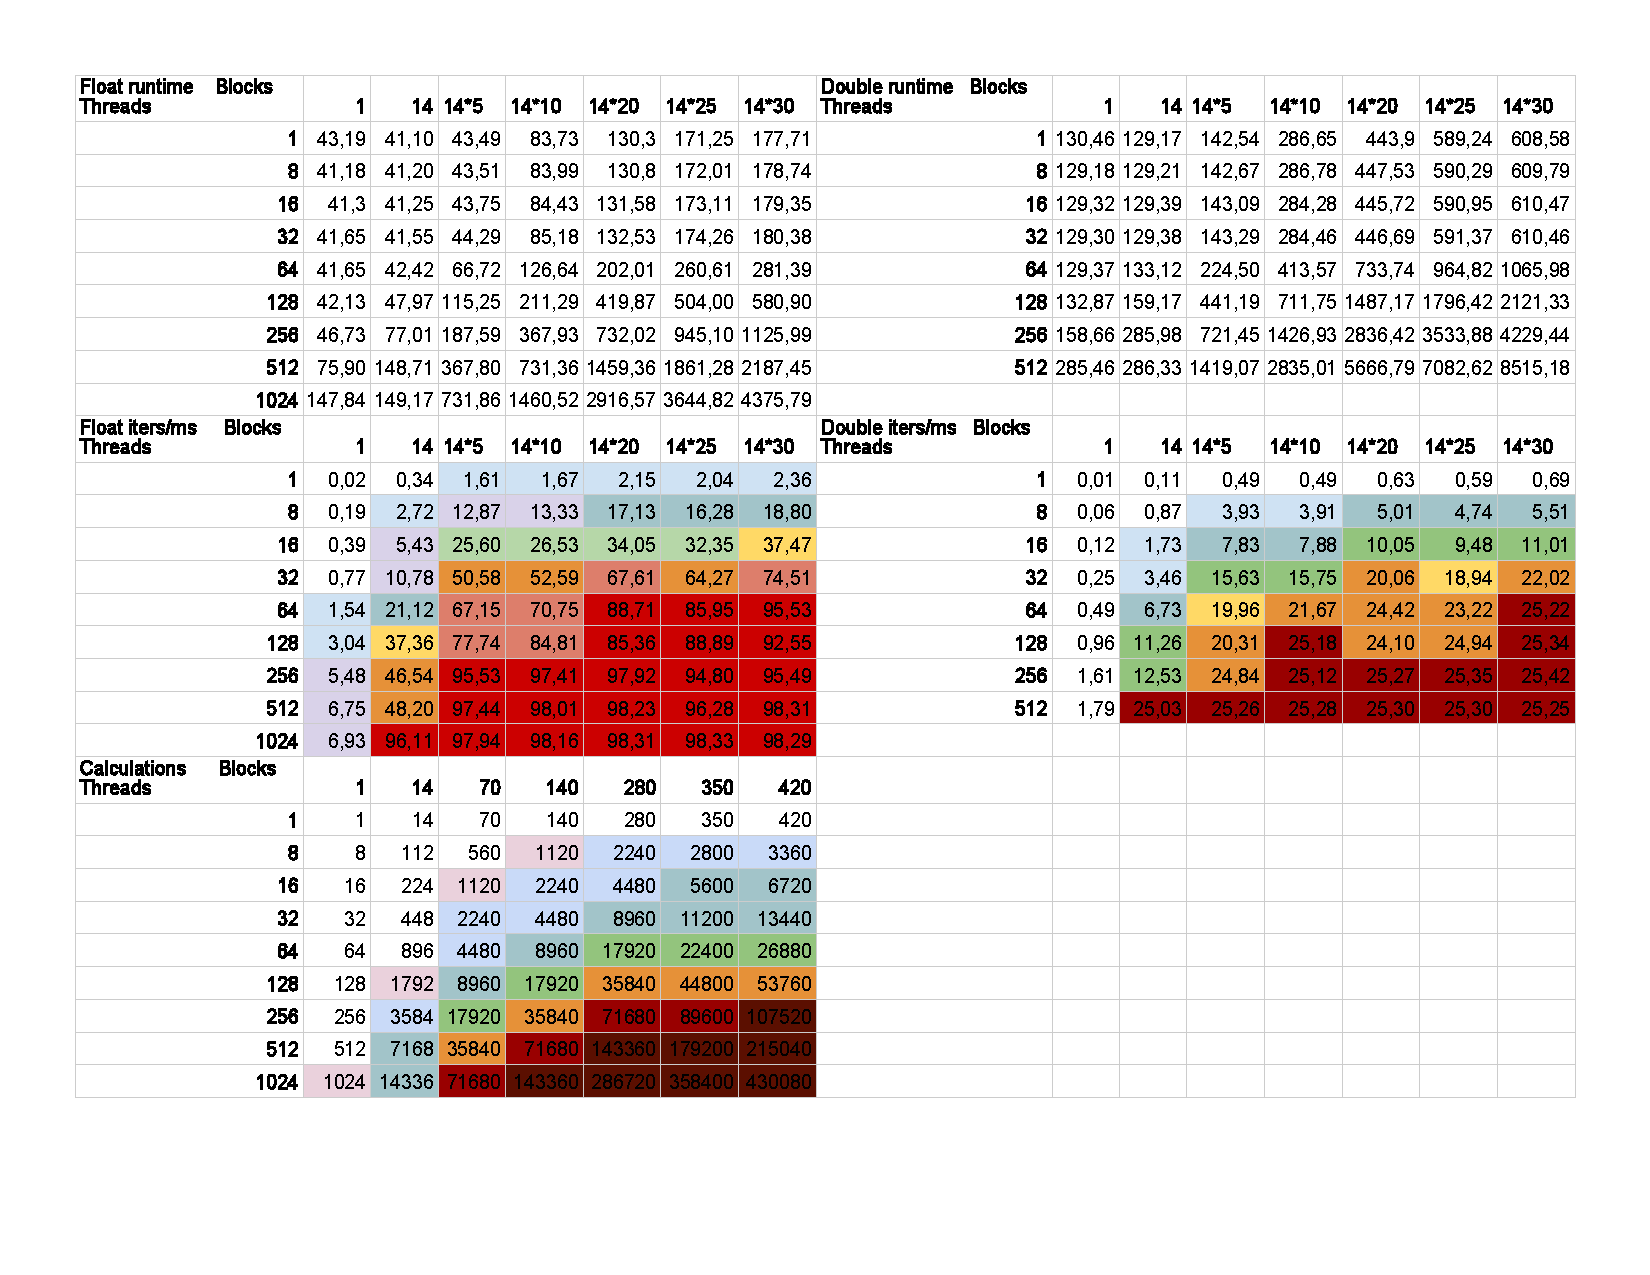
\includepdf[pages=1,angle=90,pagecommand={\section{Alea.cuBase Performance Test}\label{app:cuBase_manual_runtimes}}, frame,scale=0.65]{sections/appendix/cuBase_Manual.pdf}
  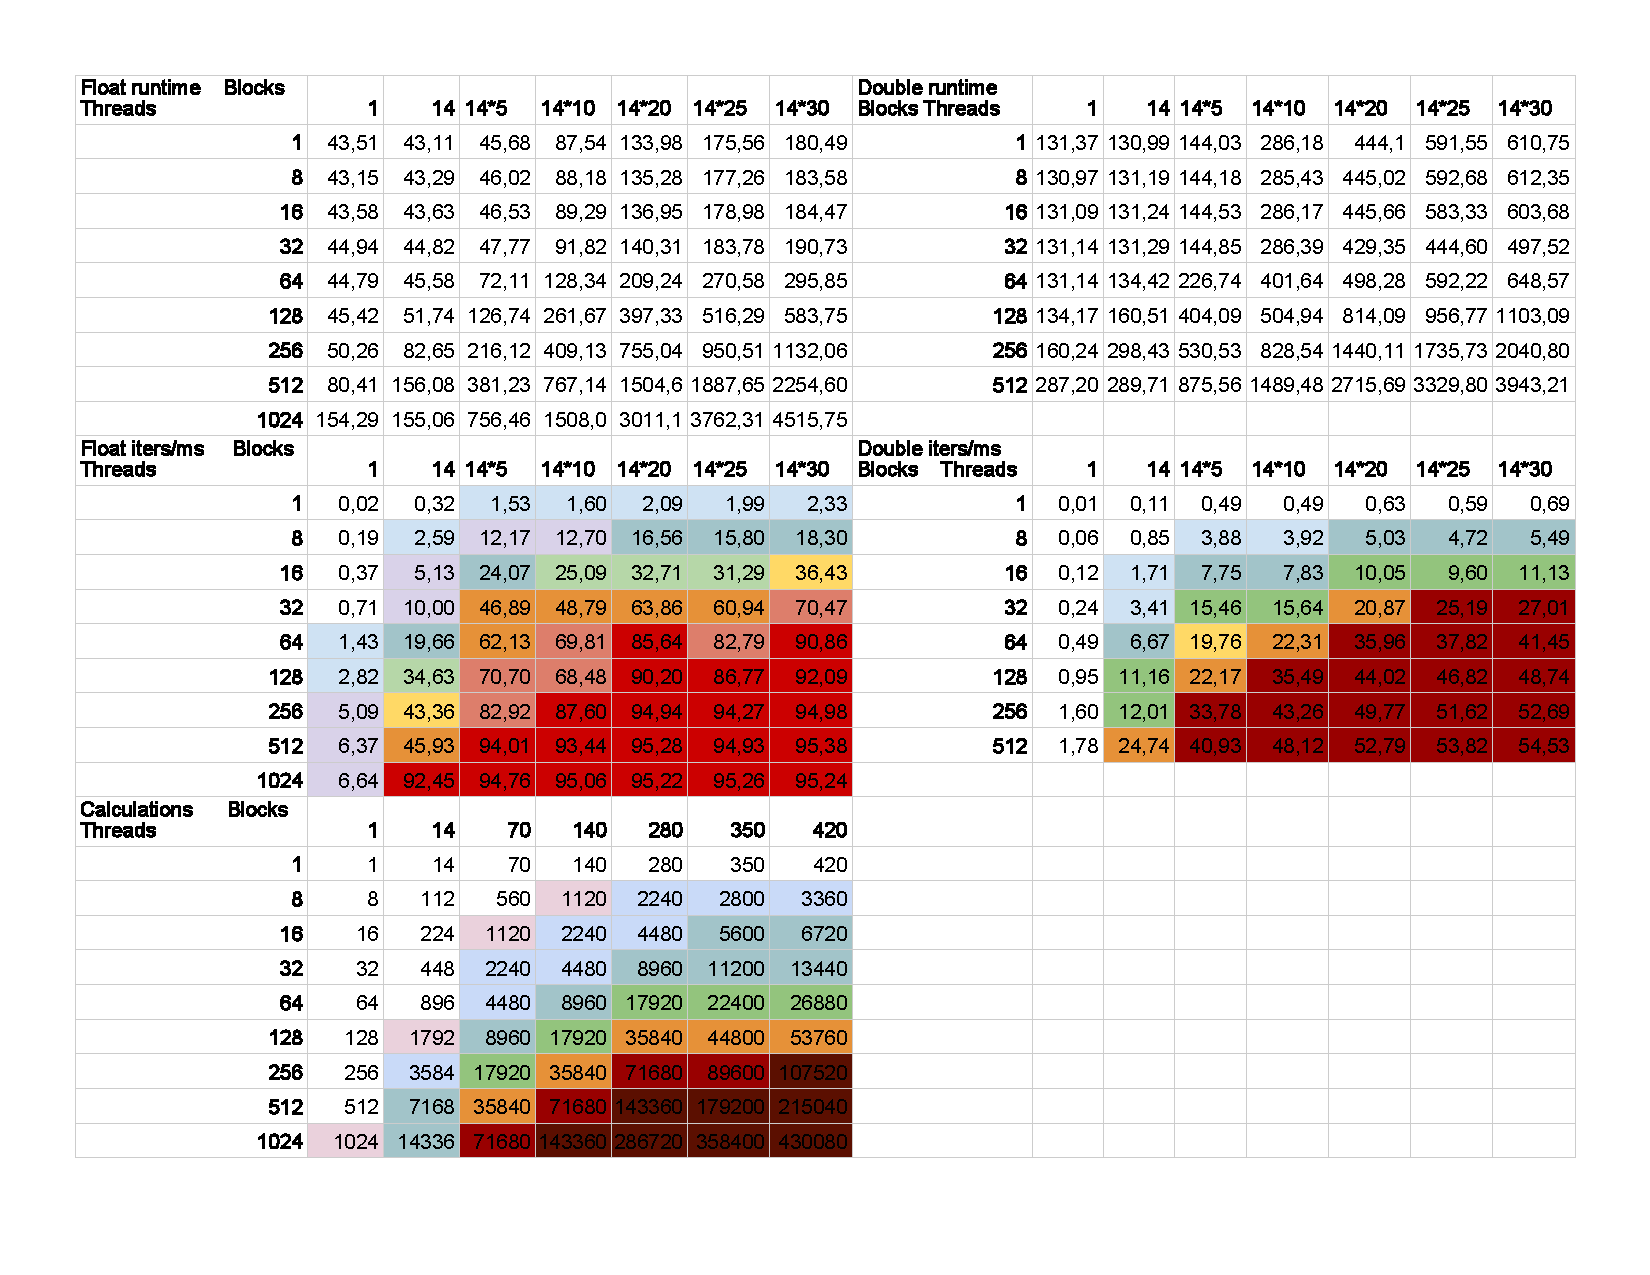
\includepdf[pages=1,angle=90,pagecommand={\section{Alea.cuBase with Params Performance Test}\label{app:cuBase_manual_params_runtimes}}, frame,scale=0.65]{sections/appendix/cuBase_Manual_Params.pdf}
  \section{C\# RK4\_n}\label{app:csharp_rk4_n}
  \lstinputlisting[language=CSharp,nolol=true]{sections/appendix/CSharp-RK4_n.txt}
  \section{Alea.cuBase RK4\_n}\label{app:cubase_rk4_n}
  \lstinputlisting[language=FSharp,nolol=true]{sections/appendix/cuBase-RK4_n.txt}
  \section{Actulus CalcSpec examples}\label{app:calcspecexamples}
  \lstinputlisting[language=CalcSpec,nolol=true]{sections/appendix/pureendowment.cs}
  \lstinputlisting[language=CalcSpec,nolol=true]{sections/appendix/deferredtemporarylifeannuity.cs}
  \lstinputlisting[language=CalcSpec,nolol=true]{sections/appendix/temporarylifeannuitypremium.cs}
  \lstinputlisting[language=CalcSpec,nolol=true]{sections/appendix/terminsurance.cs}
  \lstinputlisting[language=CalcSpec,nolol=true]{sections/appendix/disabilityannuity.cs}
  \lstinputlisting[language=CalcSpec,nolol=true]{sections/appendix/disabilityterminsurance.cs}
%\end{appendices}
